
\section{Constituencies and Counties}

\begin{enumerate}
\def\labelenumi{\arabic{enumi}.}
\itemsep1pt\parskip0pt\parsep0pt
\item
  About Wahlkreise and Landkreise
\item
  Configuration and Visualization in QGIS Desktop
\item
  Setup for Postgres (+Postgis)
\item
  Derivation of \emph{County} \textless{}-\textgreater{}
  \emph{Constituency}
\end{enumerate}

\subsection{1. About Wahlkreise and
Landkreise}\label{about-wahlkreise-and-landkreise}

\emph{{[}Description{]}}

\subsection{2. Configuration and Visualization in QGIS
Desktop}\label{configuration-and-visualization-in-qgis-desktop}

\subsubsection{Requirements}\label{requirements}

Available Layers *
\href{http://www.bundeswahlleiter.de/en/bundestagswahlen/BTW_BUND_13/wahlkreiseinteilung/kartographische_darstellung.html}{Wahlkreise}
* Download:
\href{http://www.bundeswahlleiter.de/de/bundestagswahlen/BTW_BUND_13/wahlkreiseinteilung/wahlkreisgeometrie/Geometrie_Wahlkreise_18DBT_VG1000_ETRS89.zip}{SHP}
* Projection: \textbf{EPSG:3044 - ETRS89 / ETRS-TM32} *
\href{http://www.gadm.org/country}{Landkreise} * Download
\href{http://biogeo.ucdavis.edu/data/gadm2/shp/DEU_adm.zip}{SHP} *
Projection: \textbf{EPSG:4326 - WGS84}

\subsubsection{Visualization}\label{visualization}

\begin{figure}[htbp]
\centering
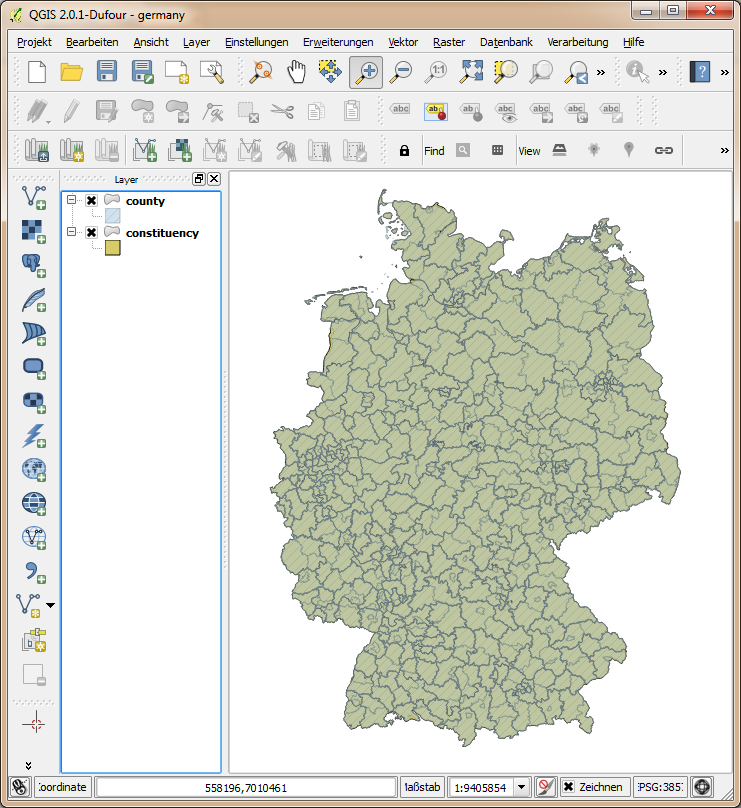
\includegraphics[width=1.1\textwidth]{../img/K4GjcyV.png}
\caption{WahlkreiseNLandkreise1}
\end{figure}

\subsubsection{Issues}\label{issues}

\begin{figure}[htbp]
\centering
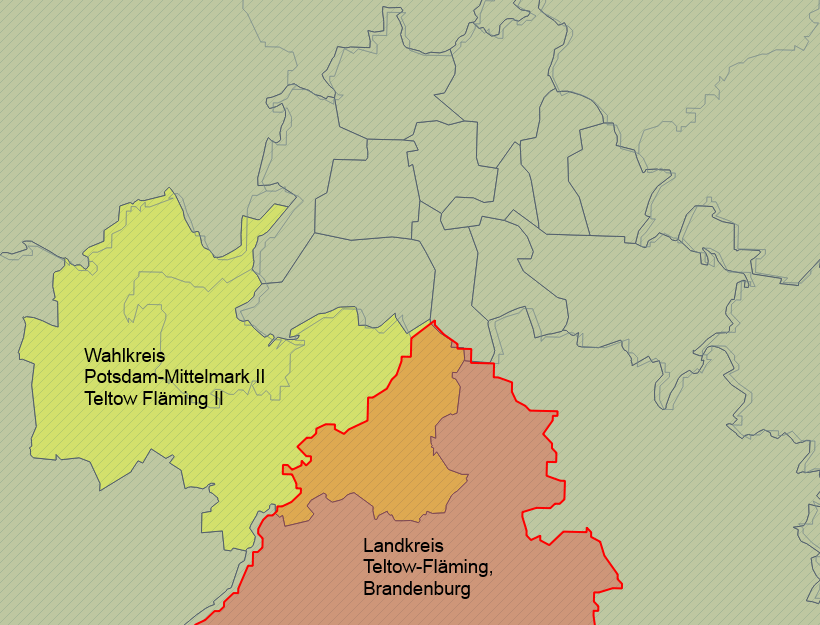
\includegraphics[width=1.1\textwidth]{../img/HdnNLcV.png}
\caption{WahlkreisVLandkreis}
\end{figure}

\begin{enumerate}
\def\labelenumi{\arabic{enumi}.}
\itemsep1pt\parskip0pt\parsep0pt
\item
  \emph{Wahlkreise} and \emph{Landkreise} are not dependent, thus their
  areas are freely intersecting each other.
\item
  \emph{Wahlkreise} and \emph{Landkreise} show a different degree of
  accuracy in position and detail when it comes to border polygons.
\end{enumerate}

\subsection{3. Setup for Postgres
(+Postgis)}\label{setup-for-postgres-postgis}

\begin{enumerate}
\def\labelenumi{\arabic{enumi}.}
\itemsep1pt\parskip0pt\parsep0pt
\item
  Import shapefiles to the database \emph{public} schema.
\end{enumerate}

\begin{itemize}
\itemsep1pt\parskip0pt\parsep0pt
\item
  \emph{Landkreise} -\textgreater{} ``county''
\item
  \emph{Wahlkreise} -\textgreater{} ``constituency''
\end{itemize}

\begin{enumerate}
\def\labelenumi{\arabic{enumi}.}
\setcounter{enumi}{1}
\itemsep1pt\parskip0pt\parsep0pt
\item
  Add two materialized SQL-Views (virtual tables) for intersections /
  dependencies between ``county'' and ``constituency'':
\end{enumerate}

xxx

\subsection{4. Derivation of \emph{County} \textless{}-\textgreater{}
\emph{Constituency}}\label{derivation-of-county---constituency}

Take \emph{Berlin} for example:

xxx

This request results in a join of intersecting counties and
constituencies, with information about the area of the participate
county, constituency and of course the intersection. A normalized
intersection \textbf{``quota''} index is calculated, which defines the
areal influence of a constituency to a county. The sum of all
constituency ``quota'' of a county is 1.

xxx

\emph{Notice:} Since the map data of constituencies and counties are
inaccurately overlapping a part of \emph{Brandenburg} constituencies
intersect with the county \emph{Berlin}. The sum of all
\textbf{``quota''} from \emph{Brandenburg} constituencies in
\emph{Berlin} county is 0.03708, which means 3.7\% of \emph{Berlin}s
area will be influenced by voting results descending from constituency
of \emph{Brandenburg}.

